% numerical.tex

\cleardoublepage
\chapter{Optimised Trajectory Including Fly-Back}\label{chapter:Flyback}

This chapter presents the optimised trajectory of the launch system, including the fly-back of the SPARTAN. The combined optimisation for the ascent/fly-back and third stage trajectory is currently operational in LODESTAR. Figures \ref{fig:ascent}-\ref{fig:groundtrack} show an example of a combined optimised trajectory for the ascent/return of the SPARTAN and the ascent of the third stage, for maximum payload-to-orbit. However, the aerodynamic and propulsive databases are currently being updated, and will change the optimised results slightly. It is not expected that the major points of interest in the trajectory will change.



 The ascent trajectory will be compared to the optimised ascent without fly-back calculated in Section \ref{chapter:Ascent}. The SPARTAN compensates for the fly-back by banking during ascent. This requires additional angle of attack, and results in less velocity and a smaller pull-up. A small deviation from 50kPa dynamic pressure is observed directly before pull-up, accompanied by a rise in bank angle. This manoeuvre reduces the total range during ascent for minimal velocity losses, decreasing the fuel necessary for the return flight. 
 

The return flight analysis consists of a modified form of the paper 'Fly-Back of a Scramjet-Powered Accelerator', presented at Scitech 2018. Currently, this analysis is for a standalone optimised fly-back from a fixed point.  The results will modified to be for the fly-back portion of the combined optimisation. The analysis in this section is expected to change little. 



The sensitivity analysis in this chapter will be expanded, and will be compared against the sensitivity analysis without fly-back, presented in Chapter \ref{chapter:Ascent}, to determine how the fly-back changes the sensitivity of the trajectory to the design parameters of the SPARTAN. As in Chapter \ref{chapter:Ascent}, the validation of each case will be discussed, with forward simulation comparisons and optimality condition validations provided in appendices. 




\section{Combined SPARTAN Ascent-Descent \& Third Stage}
\begin{table}[ht]
	\centering
\begin{tabular}{l c } 
	\hline \textbf{Trajectory Condition}
	&Standard

	\\
	\hline \textbf{Payload to Orbit (kg)}
	& \PayloadToOrbitStandard
	\\
	\textbf{Separation Alt, 1$\rightarrow$2 (km)}
	& \firstsecondSeparationAltStandard
	\\
	\textbf{Separation v, 1$\rightarrow$2 (m/s)}
	& \firstsecondSeparationvStandard
	\\
	\textbf{Separation $\gamma$, 1$\rightarrow$2 (m/s)}
	& \firstsecondSeparationgammaStandard
	\\
	\textbf{Separation Alt, 2$\rightarrow$3 (km)}
	& \secondthirdSeparationAltStandard
	\\
	\textbf{Separation $v$, 2$\rightarrow$3 (m/s)}
	& \secondthirdSeparationvStandard
	\\
	\textbf{Separation $\gamma$, 2$\rightarrow$3 (deg)}
	& \secondthirdSeparationgammaStandard
	\\
	\textbf{Separation $q$, 2$\rightarrow$3(kPa)}
	& \secondthirdSeparationqStandard
	\\
	\textbf{2$^{nd}$ Stage L/D, 2$\rightarrow$3}
	& \secondthirdSeparationLDStandard
	\\
	\textbf{2$^{nd}$ Stage Flight Time (s)}
	& \secondFlightTimeStandard
	\\
	\textbf{3$^{rd}$ Stage $t$, $q >$ 5kpa (s)}
	& \thirdqOverFiveStandard
	\\
	\textbf{3$^{rd}$ Stage max $\alpha$ (deg)}
	& \thirdmaxAoAStandard
	\\
	\textbf{3$^{rd}$ Stage final v (m/s)}
	& \thirdcircvStandard
	\\
	\textbf{3$^{rd}$ Stage final m (kg)}
	& \thirdcircmStandard
	\\
	\hline 
\end{tabular}
\end{table}

The trajectory of the rocket-scramjet-rocket launch system has been optimised in LODESTAR, including the return of the SPARTAN to its initial launch site. The optimised trajectory is shown in Figure \ref{fig:GroundTrackStandard}. The succesful computation of this optimised trajectory indicates that it is possible to launch a small satellite using the rocket-scramjet-rocket launch system, while returning the SPARTAN to the initial launch site location, and approaching the landing at appropriately low altitude and velocity. 
This optimised trajectory attains a payload mass to SSO of 173.1kg. 

The maximum payload-to-orbit is reduced by XX\% compared to the optimised trajectory result without flyback. This is a relatively small reduction in payload, and the benefits of flying back the SPARTAN to its initial launch site are likely to far outweigh this associated reduction in payload. This result indicates that flying back the SPARTAN to its initial launch site is possible, and is likely to be desirable as the most cost efficient way to operate the rocket-scramjet-rocket launch vehicle. 

The optimised trajectory shape is significantly different from that of the optimised trajectory without flyback. The initial launch is to the East, with the SPARTAN manoeuvring during its acceleration so that the heading angle is pointed close to North. The SPARTAN releases the third stage, and executes a banking turn, with a sequence of 'skipping' manoeuvres. The scramjet engine is ignited three times during the return flight, using a total of 238.3kg of fuel, 15.2\% of the total fuel mass.

\begin{figure}[ht]
	\centering
	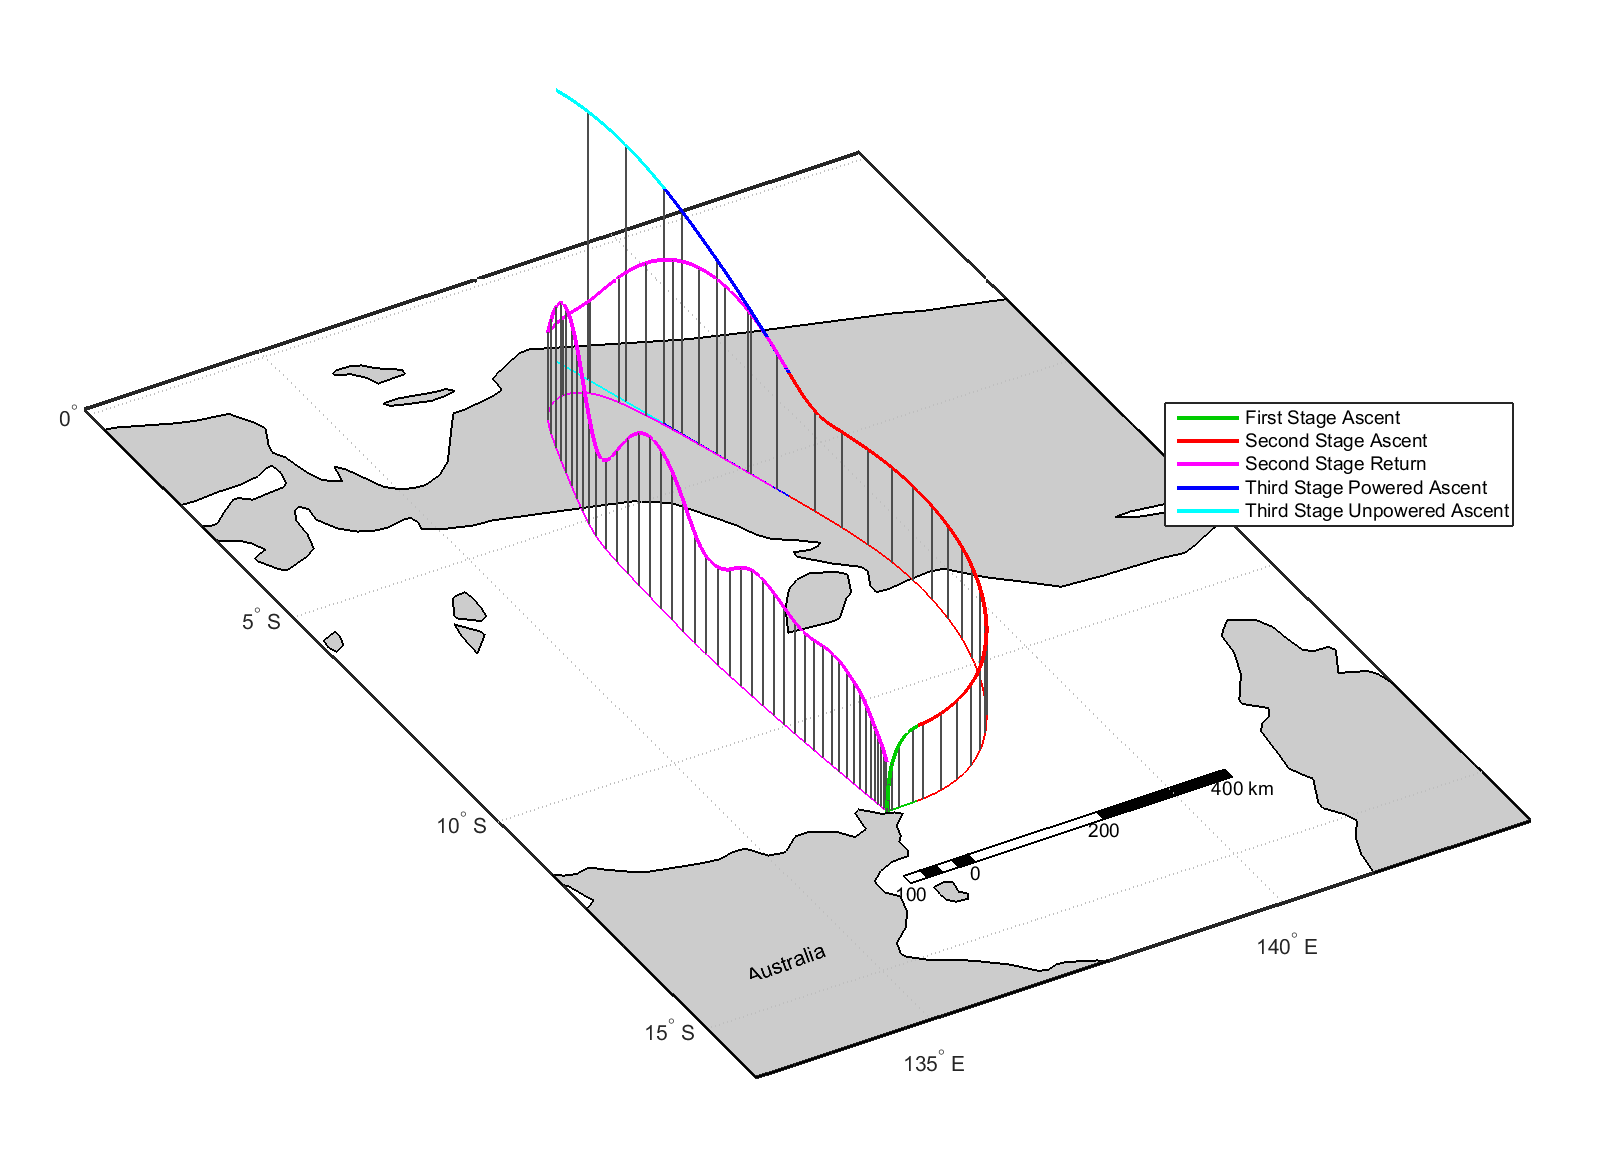
\includegraphics[width=1\linewidth]{../LODESTAR_FINAL/Results/mode11/GroundTrackStandard}
	\caption{}
	\label{fig:GroundTrackStandard}
\end{figure}

\section{First Stage Trajectory}
\begin{figure}[ht]
\centering
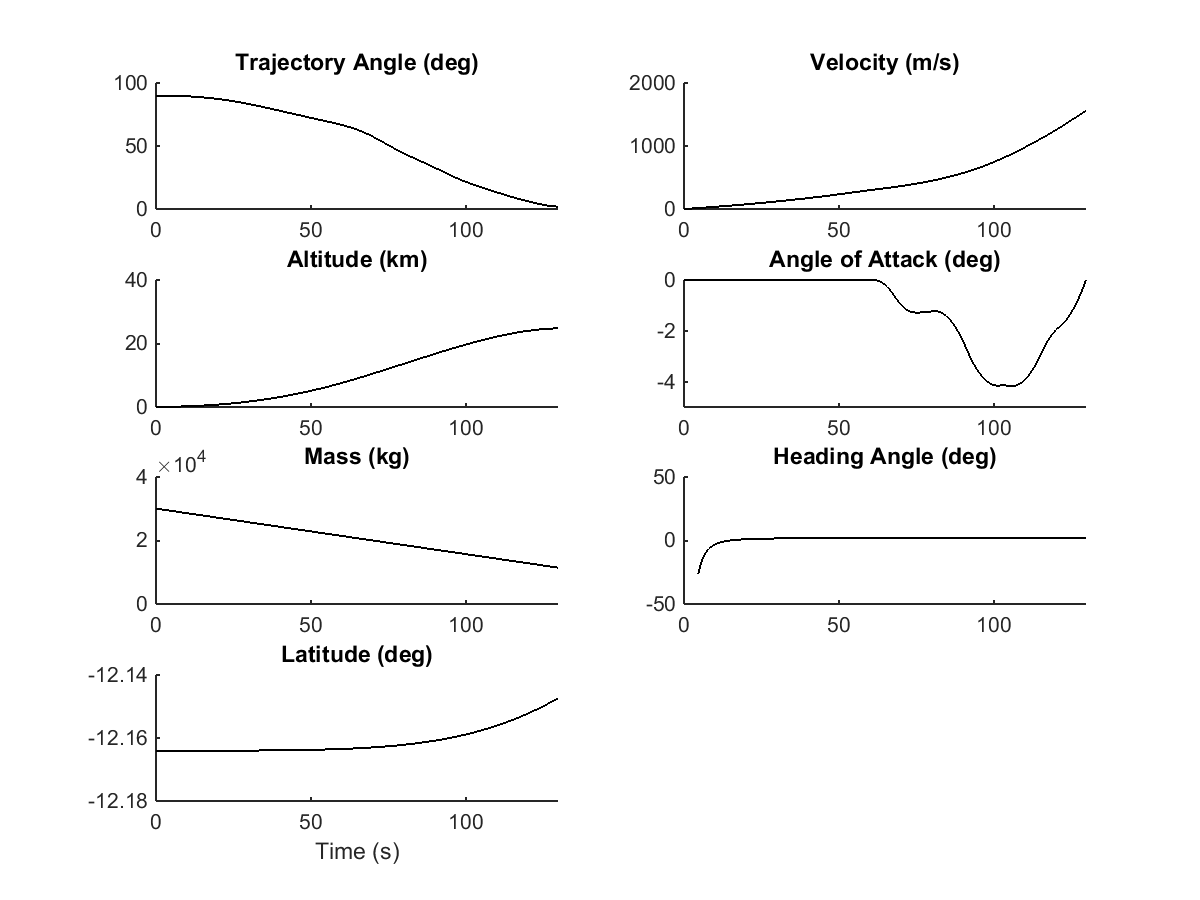
\includegraphics[width=1\linewidth]{../LODESTAR_FINAL/Results/mode11/FirstStageStandard}
\caption{}
\label{fig:FirstStageStandard}
\end{figure}

\section{Second Stage Trajectory}
\begin{figure}[ht]
\centering
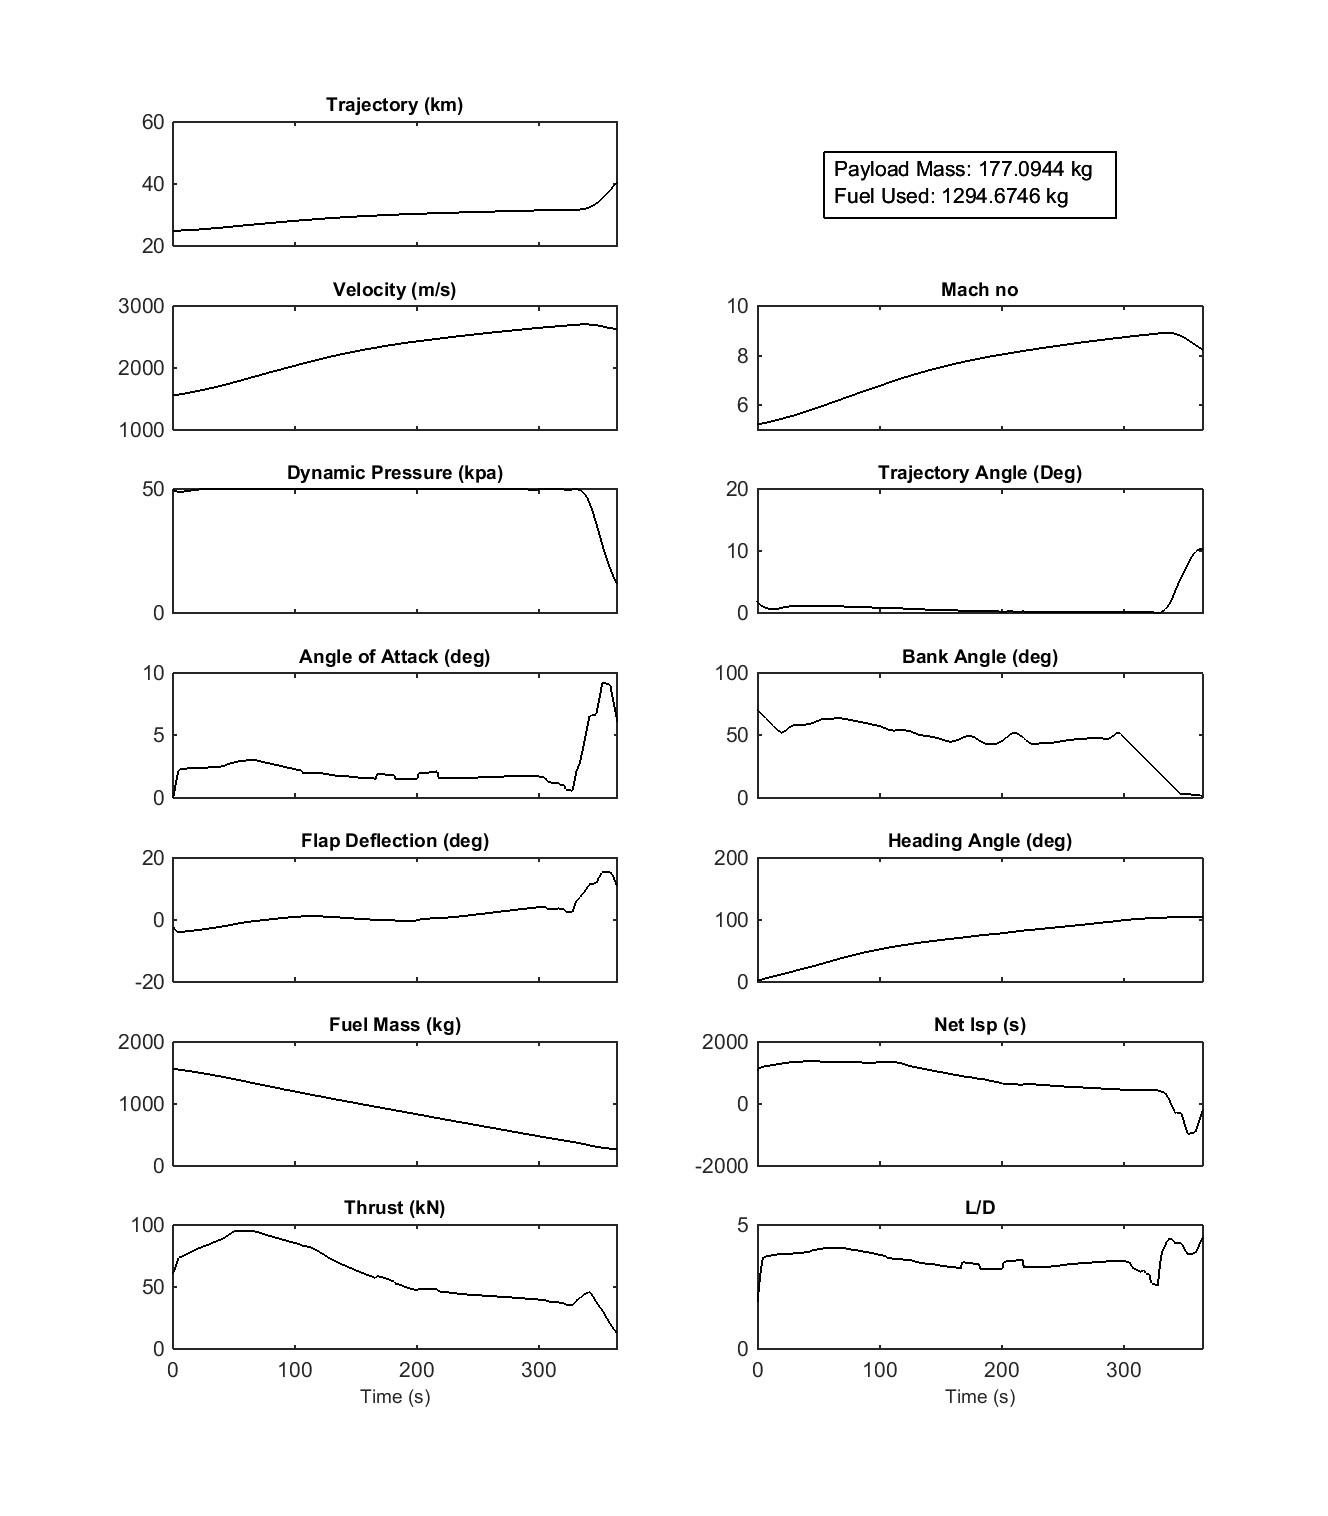
\includegraphics[width=1\linewidth]{../LODESTAR_FINAL/Results/mode11/SecondStageStandard}
\caption{}
\label{fig:SecondStageStandard}
\end{figure}

\begin{figure}[ht]
\centering
\includegraphics[width=0.9\linewidth]{../LODESTAR_FINAL/Results/mode11/NetIspStandard}
\caption{}
\label{fig:NetIspStandard}
\end{figure}



-higher AoA (maybe pinpoint location on Isp graphs)

with no return case:
-compare L/D Net Isp and thrust history

-compare end trajectory angle/altitude 

-compare eq ratio (plot of both together? dont use normalised time scale)


\section{Third Stage Trajectory}
\begin{figure}
\centering
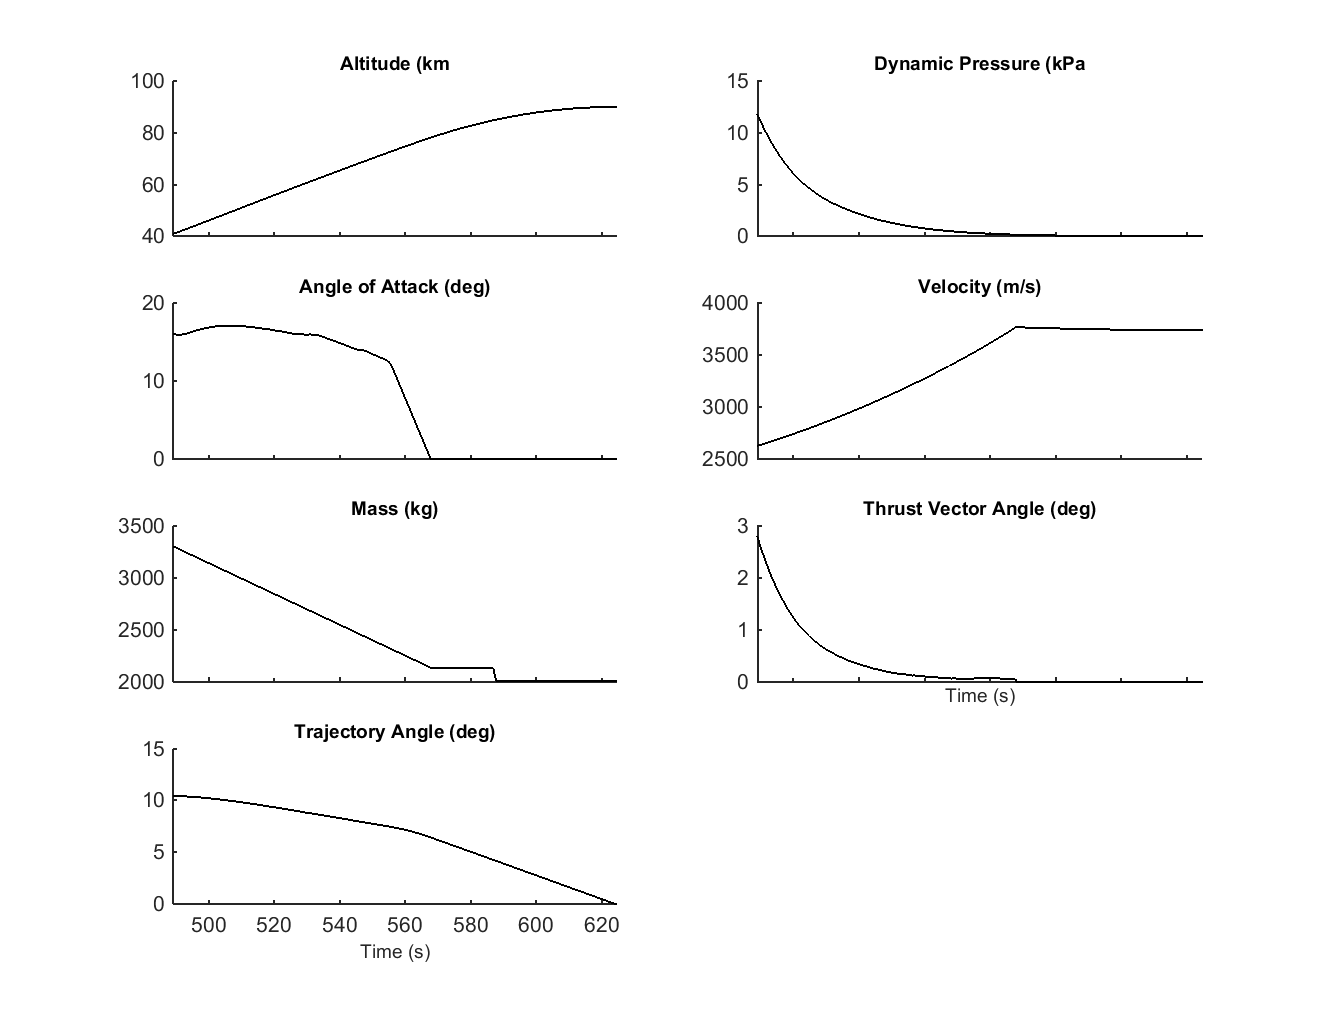
\includegraphics[width=1\linewidth]{../LODESTAR_FINAL/Results/mode11/ThirdStageStandard}
\caption{}
\label{fig:ThirdStageStandard}
\end{figure}


\section{Fly-Back Trajectory}

\begin{figure}
	\centering
	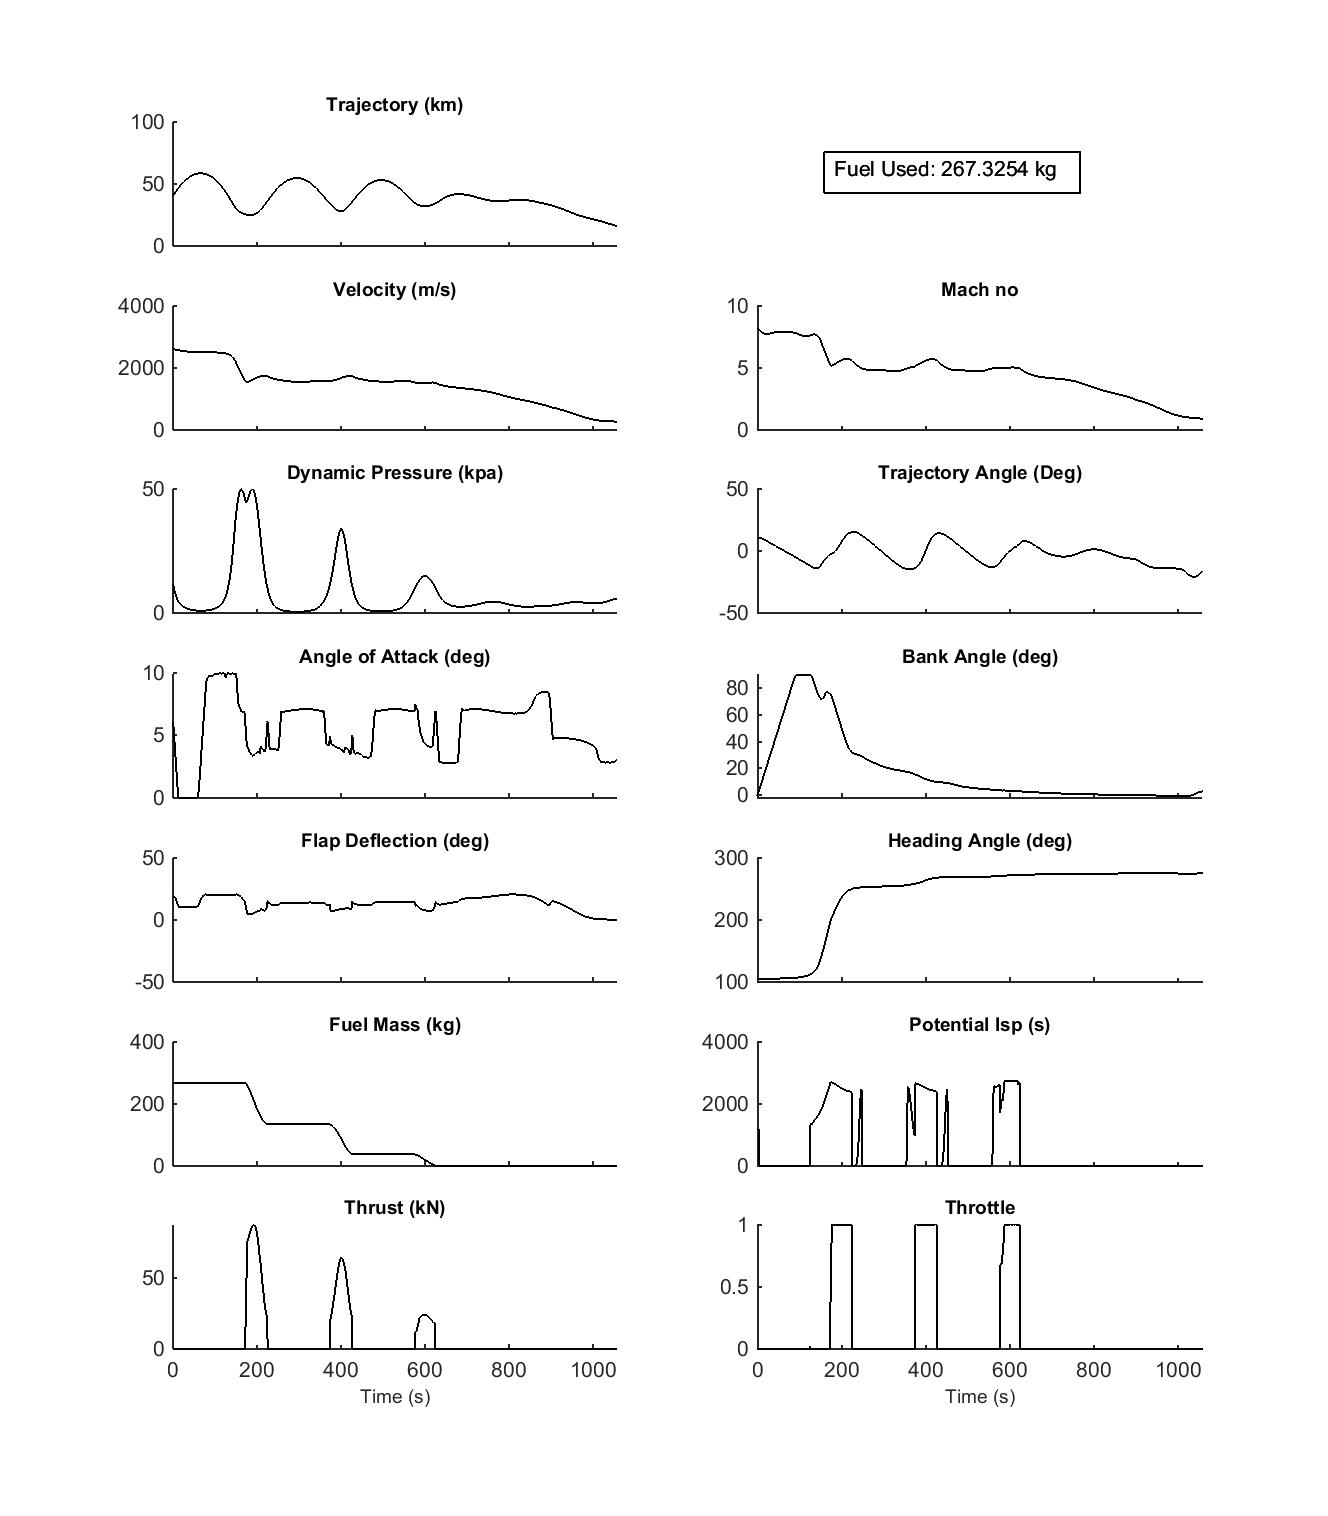
\includegraphics[width=1\linewidth]{../LODESTAR_FINAL/Results/mode11/ReturnStandard}
	\caption{}
	\label{fig:ReturnStandard}
\end{figure}

-as below, explain why the ascent banks




\section{Fly-Back Trajectory Analysis - paper}
The fly-back of the SPARTAN is optimised using LODESTAR. The fly-back is optimised for minimum fuel usage, with initial conditions constrained to be similar to the intended third stage release point, and end position constrained within 12.7km of the initial launch site, at  15.3$^\circ$S,144.9$^\circ$E\cite{ForbesSpyratos2018}. The margin of 12.7km is allowed so as to not over-constrain the end position within LODESTAR, and it is assumed that the landing strip will not be at the exact location of the launch site. The angle of attack is limited to 10$^\circ$, to ensure vehicle stability. The bank angle is limited to 90$^\circ$ to produce a conservative solution and to limit any possible design complications that may arise from inverted flight. The dynamic pressure is limited to 50kPa, the structural limit of the vehicle. The scramjet engines are limited to only operate above 20kPa dynamic pressure, an estimated lower limit on the operable mass flow rate.
The end of the trajectory is constrained to sub-200m altitude, and a trajectory angle range between -10$^\circ$ and 0$^\circ$ to ensure that the SPARTAN can perform a landing manoeuvre. These constraints ensure that the vehicle is approaching the landing site at the end of the optimised trajectory. The end velocity is only limited to be greater than 0m/s. It can be assumed that the optimal fly-back trajectory minimises end velocity as shown in the optimised trajectory results. 
It is also assumed that the vehicle is able to carry any necessary fuel in addition to the fuel required during the ascent trajectory, allowing the initial conditions to be kept constant. The potential specific impulse is shown along the trajectory, this is the specific impulse obtainable from the C-REST engines should they be powered on.




\subsection{Return Trajectory}


The optimised fly-back trajectory is shown in Figures \ref{fig:lon-lat} and \ref{fig:AllTraj}.
The fly-back is initiated from the optimised second-third stage separation point at 7.7$^\circ$S,145.0$^\circ$E, 34.5km altitude, 2.9$^\circ$ trajectory angle, 2881m/s velocity and 102$^\circ$ heading angle, corresponding to the conditions of optimal third stage release described in Section \ref*{sec:opt}. 
The SPARTAN is shown to be capable of fly-back, using 166.0kg of fuel, a total increase in the fuel usage of the SPARTAN of 10.6\%.
The optimised trajectory has four distinct parts; 1. initial turn, 2. boost phase, 3. hop-glide, and 4. approach. 

\subsubsection{ Initial Turn}
The SPARTAN starts at the maximum bank angle of 90$^\circ$, and sustains this bank angle for 34.4s. At this point, the altitude of the SPARTAN decreases, and the vehicle is close to hitting the dynamic pressure of 50kPa. To avoid exceeding this limit, the bank angle is reduced to 71.2$^\circ$, allowing the vehicle to generate sufficient lift to slow its descent. The bank angle in then increased again, to 80.7$^\circ$ at 70.8s. After this time, the bank angle is gradually reduced. 

\subsubsection{ Boost Phase}
Soon after the bank angle begins to reduce, at 118.7s flight time and Mach 5.71, the scramjet engines are ignited. The C-REST engines are powered-on at a point of high potential specific impulse, at a low Mach number, and burn for 119.8s. The altitude of the SPARTAN is raised during the majority of the burn, ensuring that the Mach number is kept low for maximum efficiency\cite{Preller2017}, as shown in Figure \ref{fig:AllTraj}. The maximum altitude is limited by the lower dynamic pressure limit of the C-REST engines of 20kPa. The bank angle of the vehicle is reduced to produce increased lift, so as to increase the altitude of the SPARTAN, while also maximising the specific impulse of the scramjet engines by keeping the angle of attack low. Low angle of attack decreases the temperature and raises the Mach number, at the inlet of the C-REST engines. While these effects partially offset each other\cite{Preller2017}, the temperature increase is more significant, and decreasing angle of attack has the net effect of increasing the specific impulse of the C-REST engines. This increase in specific impulse is balanced by a decrease in the L/D of the SPARTAN at angle of attack values lower than 4$^\circ$, as illustrated in Figure \ref{fig:LD}. However, the specific impulse has a more significant impact than L/D during this phase, resulting in the optimised angle of attack being kept low. At 204s the angle of attack is increased, bringing the L/D of the vehicle towards maximum and initiating the first 'skip' of the skip-glide phase.  


\subsubsection{ Skip-Glide}
During the unpowered trajectory after the burn phase, the angle of attack is controlled so that the L/D of the SPARTAN is close to the maximum. Initially, the SPARTAN performs several 'skips' after the scramjet burn. These are due to the high L/D of the SPARTAN above Mach 4, and are aided by the angle of attack, which is controlled to emphasize the size of the skips. These skips are consistent with research which has shown that a periodic skipping trajectory increases the downrange distance achievable by hypersonic vehicles\cite{Eggers1957,Kanda2007}. 


\subsubsection{ Approach}
After the skip phase, as the vehicle is approaching Mach 1, the angle of attack is reduced gradually to bring the SPARTAN down to 1km altitude, in a controlled manner. 
At the end of the trajectory the SPARTAN levels out, and reaches 1km altitude at -XX$^\circ$ trajectory angle and XXm/s velocity. These conditions are similar to those of the space shuttle at landing\cite{Ryba2017}, and it is assumed that the SPARTAN is able to perform a landing manoeuvre after this point. 








\subsection{Design Sensitivity Analysis}

During the preliminary stages of launch vehicle design, it is important to characterise the effects of changes in the design of a vehicle.  
Quantifying the effects of variations within the vehicle design allows the vehicle performance to be improved. 
However, the complete assessment of the effects of vehicle design variations requires every critical feature of the design to be modified, and the new vehicle design to be investigated. This method of investigation is prohibitively time consuming and computationally expensive for a complex launch system. Consequently, it is important to first understand the effects of the key performance parameters of the vehicle, so that when the design of the launch system is to be iterated, the design of each vehicle and subsystem may be tailored towards improving the overall performance.
 The this end, a sensitivity study is performed to investigate the variations in the optimal trajectory when key performance parameters of the vehicle are modified.

The performance parameters modified are:

\begin{itemize}
	\item Maximum dynamic pressure.
	\item Specific Impulse of the C-REST engines. 
	\item SPARTAN aerodynamic drag.
	\item SPARTAN mass.
	\item SPARTAN fuel mass.
	\item Third stage mass.
	\item Third stage thrust. 
	\item SPARTAN viscous drag. 
	
\end{itemize}



 These parameters are varied and the new optimal fly-back trajectories are calculated using LODESTAR. These optimised trajectories are detailed in the following sections.
 
The consistency of the trajectory shape indicates that the optimal solution is robust with variation in the aerodynamic parameters and specific impulse of the SPARTAN. The optimised trajectories show clear trends with variation in vehicle parameters.






\section{dynamic pressure}



\begin{table}[ht]
\centering

\end{table}


\section{Isp}


Increasing the specific impulse causes the fuel necessary for fly-back to decrease by -XXkg (-XX\%), while decreasing the specific impulse causes the fuel necessary to rise by +XXkg (+XX\%). The start of scramjet burn is consistent across different specific impulse test cases. Due to the increase in thrust, the SPARTAN accelerates more rapidly for the higher specific impulse case. As a consequence, the initial 'skip' is performed sooner, and subsequent skips are larger. 

-check this

\begin{table}[ht]
	\centering
	\begin{tabular}{l c c c c c c} 
		\hline \textbf{Trajectory Condition}
		&Isp90
		&Isp95
		&Isp100
		&Isp105
		&Isp110
		& /\%
		\\
		\hline \textbf{Payload to Orbit (kg)}
		& \PayloadToOrbitIspNinety
		& \PayloadToOrbitIspNinetyFive
		& \PayloadToOrbitIspStandard
		& \PayloadToOrbitIspOneHundredFive
		& \PayloadToOrbitIspOneHundredTen
		&1.7
		\\
		\textbf{Separation Alt, 1$\rightarrow$2 (km)}
		& \firstsecondSeparationAltIspNinety
		& \firstsecondSeparationAltIspNinetyFive
		& \firstsecondSeparationAltIspStandard
		& \firstsecondSeparationAltIspOneHundredFive
		& \firstsecondSeparationAltIspOneHundredTen
		& -
		\\
		\textbf{Separation v, 1$\rightarrow$2 (m/s)}
		& \firstsecondSeparationvIspNinety
		& \firstsecondSeparationvIspNinetyFive
		& \firstsecondSeparationvIspStandard
		& \firstsecondSeparationvIspOneHundredFive
		& \firstsecondSeparationvIspOneHundredTen
		& -
		\\
		\textbf{Separation $\gamma$, 1$\rightarrow$2 (m/s)}
		& \firstsecondSeparationgammaIspNinety
		& \firstsecondSeparationgammaIspNinetyFive
		& \firstsecondSeparationgammaIspStandard
		& \firstsecondSeparationgammaIspOneHundredFive
		& \firstsecondSeparationgammaIspOneHundredTen
		& -
		\\
		\textbf{Separation Alt, 2$\rightarrow$3 (km)}
		& \secondthirdSeparationAltIspNinety
		& \secondthirdSeparationAltIspNinetyFive
		& \secondthirdSeparationAltIspStandard
		& \secondthirdSeparationAltIspOneHundredFive
		& \secondthirdSeparationAltIspOneHundredTen
		& -
		\\
		\textbf{Separation $v$, 2$\rightarrow$3 (m/s)}
		& \secondthirdSeparationvIspNinety
		& \secondthirdSeparationvIspNinetyFive
		& \secondthirdSeparationvIspStandard
		& \secondthirdSeparationvIspOneHundredFive
		& \secondthirdSeparationvIspOneHundredTen
		&11.1
		\\
		\textbf{Separation $\gamma$, 2$\rightarrow$3 (deg)}
		& \secondthirdSeparationgammaIspNinety
		& \secondthirdSeparationgammaIspNinetyFive
		& \secondthirdSeparationgammaIspStandard
		& \secondthirdSeparationgammaIspOneHundredFive
		& \secondthirdSeparationgammaIspOneHundredTen
		&-0.09
		\\
		\textbf{Separation $q$, 2$\rightarrow$3(kPa)}
		& \secondthirdSeparationqIspNinety
		& \secondthirdSeparationqIspNinetyFive
		& \secondthirdSeparationqIspStandard
		& \secondthirdSeparationqIspOneHundredFive
		& \secondthirdSeparationqIspOneHundredTen
		&0.06
		\\
		\textbf{2$^{nd}$ Stage L/D, 2$\rightarrow$3}
		& \secondthirdSeparationLDIspNinety
		& \secondthirdSeparationLDIspNinetyFive
		& \secondthirdSeparationLDIspStandard
		& \secondthirdSeparationLDIspOneHundredFive
		& \secondthirdSeparationLDIspOneHundredTen
		& -
		\\
		\textbf{2$^{nd}$ Stage Flight Time (s)}
		& \secondFlightTimeIspNinety
		& \secondFlightTimeIspNinetyFive
		& \secondFlightTimeIspStandard
		& \secondFlightTimeIspOneHundredFive
		& \secondFlightTimeIspOneHundredTen
		& -
		\\
		\textbf{3$^{rd}$ Stage $t$, $q >$ 5kpa (s)}
		& \thirdqOverFiveIspNinety
		& \thirdqOverFiveIspNinetyFive
		& \thirdqOverFiveIspStandard
		& \thirdqOverFiveIspOneHundredFive
		& \thirdqOverFiveIspOneHundredTen
		& -
		\\
		\textbf{3$^{rd}$ Stage max $\alpha$ (deg)}
		& \thirdmaxAoAIspNinety
		& \thirdmaxAoAIspNinetyFive
		& \thirdmaxAoAIspStandard
		& \thirdmaxAoAIspOneHundredFive
		& \thirdmaxAoAIspOneHundredTen
		& -
		\\
		\textbf{3$^{rd}$ Stage final v (m/s)}
		& \thirdcircvIspNinety
		& \thirdcircvIspNinetyFive
		& \thirdcircvIspStandard
		& \thirdcircvIspOneHundredFive
		& \thirdcircvIspOneHundredTen
		&12.46
		\\
		\textbf{3$^{rd}$ Stage final m (kg)}
		& \thirdcircmIspNinety
		& \thirdcircmIspNinetyFive
		& \thirdcircmIspStandard
		& \thirdcircmIspOneHundredFive
		& \thirdcircmIspOneHundredTen
		& -
		\\
		\hline 
	\end{tabular} 
	
\end{table}

\section{Cd}

Increasing the drag coefficient causes the fuel necessary for fly-back to increase by +XXkg (+XX\%). Conversely, decreasing the drag coefficient by 10\% causes the fuel necessary for  fly-back to decrease by -XXkg (-XX\%). 
When the drag is increased (ie. L/D is decreased), the scramjet engine burn phase begins earlier, and continues for longer. 
The greater burn time allows the maximum altitude attained during the initial 'skip' to be higher. 
This additional altitude is necessary as the greater drag causes the velocity, and consequentially altitude, of the SPARTAN to decrease more rapidly.

-check all this

\begin{table}[ht]
	\centering
	\begin{tabular}{l c c c c c c} 
		\hline \textbf{Trajectory Condition}
		&Cd90
		&Cd95
		&Cd100
		&Cd105
		&Cd110
		& /\%
		\\
		\hline \textbf{Payload to Orbit (kg)}
		& \PayloadToOrbitCdNinety
		& \PayloadToOrbitCdNinetyFive
		& \PayloadToOrbitCdStandard
		& \PayloadToOrbitCdOneHundredFive
		& \PayloadToOrbitCdOneHundredTen
		&-1.6
		\\
		\textbf{Separation Alt, 1$\rightarrow$2 (km)}
		& \firstsecondSeparationAltCdNinety
		& \firstsecondSeparationAltCdNinetyFive
		& \firstsecondSeparationAltCdStandard
		& \firstsecondSeparationAltCdOneHundredFive
		& \firstsecondSeparationAltCdOneHundredTen
		& -
		\\
		\textbf{Separation v, 1$\rightarrow$2 (m/s)}
		& \firstsecondSeparationvCdNinety
		& \firstsecondSeparationvCdNinetyFive
		& \firstsecondSeparationvCdStandard
		& \firstsecondSeparationvCdOneHundredFive
		& \firstsecondSeparationvCdOneHundredTen
		&-3.67
		\\
		\textbf{Separation $\gamma$, 1$\rightarrow$2 (m/s)}
		& \firstsecondSeparationgammaCdNinety
		& \firstsecondSeparationgammaCdNinetyFive
		& \firstsecondSeparationgammaCdStandard
		& \firstsecondSeparationgammaCdOneHundredFive
		& \firstsecondSeparationgammaCdOneHundredTen
		& -
		\\
		\textbf{Separation Alt, 2$\rightarrow$3 (km)}
		& \secondthirdSeparationAltCdNinety
		& \secondthirdSeparationAltCdNinetyFive
		& \secondthirdSeparationAltCdStandard
		& \secondthirdSeparationAltCdOneHundredFive
		& \secondthirdSeparationAltCdOneHundredTen
		&-0.07
		\\
		\textbf{Separation $v$, 2$\rightarrow$3 (m/s)}
		& \secondthirdSeparationvCdNinety
		& \secondthirdSeparationvCdNinetyFive
		& \secondthirdSeparationvCdStandard
		& \secondthirdSeparationvCdOneHundredFive
		& \secondthirdSeparationvCdOneHundredTen
		&-9.75
		\\
		\textbf{Separation $\gamma$, 2$\rightarrow$3 (deg)}
		& \secondthirdSeparationgammaCdNinety
		& \secondthirdSeparationgammaCdNinetyFive
		& \secondthirdSeparationgammaCdStandard
		& \secondthirdSeparationgammaCdOneHundredFive
		& \secondthirdSeparationgammaCdOneHundredTen
		&0.05
		\\
		\textbf{Separation $q$, 2$\rightarrow$3(kPa)}
		& \secondthirdSeparationqCdNinety
		& \secondthirdSeparationqCdNinetyFive
		& \secondthirdSeparationqCdStandard
		& \secondthirdSeparationqCdOneHundredFive
		& \secondthirdSeparationqCdOneHundredTen
		& -
		\\
		\textbf{2$^{nd}$ Stage L/D, 2$\rightarrow$3}
		& \secondthirdSeparationLDCdNinety
		& \secondthirdSeparationLDCdNinetyFive
		& \secondthirdSeparationLDCdStandard
		& \secondthirdSeparationLDCdOneHundredFive
		& \secondthirdSeparationLDCdOneHundredTen
		& -
		\\
		\textbf{2$^{nd}$ Stage Flight Time (s)}
		& \secondFlightTimeCdNinety
		& \secondFlightTimeCdNinetyFive
		& \secondFlightTimeCdStandard
		& \secondFlightTimeCdOneHundredFive
		& \secondFlightTimeCdOneHundredTen
		& -
		\\
		\textbf{3$^{rd}$ Stage $t$, $q >$ 5kpa (s)}
		& \thirdqOverFiveCdNinety
		& \thirdqOverFiveCdNinetyFive
		& \thirdqOverFiveCdStandard
		& \thirdqOverFiveCdOneHundredFive
		& \thirdqOverFiveCdOneHundredTen
		& -
		\\
		\textbf{3$^{rd}$ Stage max $\alpha$ (deg)}
		& \thirdmaxAoACdNinety
		& \thirdmaxAoACdNinetyFive
		& \thirdmaxAoACdStandard
		& \thirdmaxAoACdOneHundredFive
		& \thirdmaxAoACdOneHundredTen
		& -
		\\
		\textbf{3$^{rd}$ Stage final v (m/s)}
		& \thirdcircvCdNinety
		& \thirdcircvCdNinetyFive
		& \thirdcircvCdStandard
		& \thirdcircvCdOneHundredFive
		& \thirdcircvCdOneHundredTen
		&-7.99
		\\
		\textbf{3$^{rd}$ Stage final m (kg)}
		& \thirdcircmCdNinety
		& \thirdcircmCdNinetyFive
		& \thirdcircmCdStandard
		& \thirdcircmCdOneHundredFive
		& \thirdcircmCdOneHundredTen
		& -
		\\
		\hline 
	\end{tabular} 
\end{table}


\section{m SPARTAN}


\begin{table}[ht]
\centering
\begin{tabular}{l c c c c c c} 
	\hline \textbf{Trajectory Condition}
	&m295
	&m297.5
	&m2100
	&m2102.5
	&m2105
	& /\%
	\\
	\hline \textbf{Payload to Orbit (kg)}
	& \PayloadToOrbitmSPARTANNinetyFive
	& \PayloadToOrbitmSPARTANNinetySevenFive
	& \PayloadToOrbitmSPARTANStandard
	& \PayloadToOrbitmSPARTANOneHundredTwoFive
	& \PayloadToOrbitmSPARTANOneHundredFive
	&-1.2
	\\
	\textbf{Separation Alt, 1$\rightarrow$2 (km)}
	& \firstsecondSeparationAltmSPARTANNinetyFive
	& \firstsecondSeparationAltmSPARTANNinetySevenFive
	& \firstsecondSeparationAltmSPARTANStandard
	& \firstsecondSeparationAltmSPARTANOneHundredTwoFive
	& \firstsecondSeparationAltmSPARTANOneHundredFive
	& -
	\\
	\textbf{Separation v, 1$\rightarrow$2 (m/s)}
	& \firstsecondSeparationvmSPARTANNinetyFive
	& \firstsecondSeparationvmSPARTANNinetySevenFive
	& \firstsecondSeparationvmSPARTANStandard
	& \firstsecondSeparationvmSPARTANOneHundredTwoFive
	& \firstsecondSeparationvmSPARTANOneHundredFive
	&-8.09
	\\
	\textbf{Separation $\gamma$, 1$\rightarrow$2 (m/s)}
	& \firstsecondSeparationgammamSPARTANNinetyFive
	& \firstsecondSeparationgammamSPARTANNinetySevenFive
	& \firstsecondSeparationgammamSPARTANStandard
	& \firstsecondSeparationgammamSPARTANOneHundredTwoFive
	& \firstsecondSeparationgammamSPARTANOneHundredFive
	& -
	\\
	\textbf{Separation Alt, 2$\rightarrow$3 (km)}
	& \secondthirdSeparationAltmSPARTANNinetyFive
	& \secondthirdSeparationAltmSPARTANNinetySevenFive
	& \secondthirdSeparationAltmSPARTANStandard
	& \secondthirdSeparationAltmSPARTANOneHundredTwoFive
	& \secondthirdSeparationAltmSPARTANOneHundredFive
	& -
	\\
	\textbf{Separation $v$, 2$\rightarrow$3 (m/s)}
	& \secondthirdSeparationvmSPARTANNinetyFive
	& \secondthirdSeparationvmSPARTANNinetySevenFive
	& \secondthirdSeparationvmSPARTANStandard
	& \secondthirdSeparationvmSPARTANOneHundredTwoFive
	& \secondthirdSeparationvmSPARTANOneHundredFive
	&-7.47
	\\
	\textbf{Separation $\gamma$, 2$\rightarrow$3 (deg)}
	& \secondthirdSeparationgammamSPARTANNinetyFive
	& \secondthirdSeparationgammamSPARTANNinetySevenFive
	& \secondthirdSeparationgammamSPARTANStandard
	& \secondthirdSeparationgammamSPARTANOneHundredTwoFive
	& \secondthirdSeparationgammamSPARTANOneHundredFive
	& -
	\\
	\textbf{Separation $q$, 2$\rightarrow$3(kPa)}
	& \secondthirdSeparationqmSPARTANNinetyFive
	& \secondthirdSeparationqmSPARTANNinetySevenFive
	& \secondthirdSeparationqmSPARTANStandard
	& \secondthirdSeparationqmSPARTANOneHundredTwoFive
	& \secondthirdSeparationqmSPARTANOneHundredFive
	& -
	\\
	\textbf{2$^{nd}$ Stage L/D, 2$\rightarrow$3}
	& \secondthirdSeparationLDmSPARTANNinetyFive
	& \secondthirdSeparationLDmSPARTANNinetySevenFive
	& \secondthirdSeparationLDmSPARTANStandard
	& \secondthirdSeparationLDmSPARTANOneHundredTwoFive
	& \secondthirdSeparationLDmSPARTANOneHundredFive
	& -
	\\
	\textbf{2$^{nd}$ Stage Flight Time (s)}
	& \secondFlightTimemSPARTANNinetyFive
	& \secondFlightTimemSPARTANNinetySevenFive
	& \secondFlightTimemSPARTANStandard
	& \secondFlightTimemSPARTANOneHundredTwoFive
	& \secondFlightTimemSPARTANOneHundredFive
	& -
	\\
	\textbf{3$^{rd}$ Stage $t$, $q >$ 5kpa (s)}
	& \thirdqOverFivemSPARTANNinetyFive
	& \thirdqOverFivemSPARTANNinetySevenFive
	& \thirdqOverFivemSPARTANStandard
	& \thirdqOverFivemSPARTANOneHundredTwoFive
	& \thirdqOverFivemSPARTANOneHundredFive
	& -
	\\
	\textbf{3$^{rd}$ Stage max $\alpha$ (deg)}
	& \thirdmaxAoAmSPARTANNinetyFive
	& \thirdmaxAoAmSPARTANNinetySevenFive
	& \thirdmaxAoAmSPARTANStandard
	& \thirdmaxAoAmSPARTANOneHundredTwoFive
	& \thirdmaxAoAmSPARTANOneHundredFive
	& -
	\\
	\textbf{3$^{rd}$ Stage final v (m/s)}
	& \thirdcircvmSPARTANNinetyFive
	& \thirdcircvmSPARTANNinetySevenFive
	& \thirdcircvmSPARTANStandard
	& \thirdcircvmSPARTANOneHundredTwoFive
	& \thirdcircvmSPARTANOneHundredFive
	& -
	\\
	\textbf{3$^{rd}$ Stage final m (kg)}
	& \thirdcircmmSPARTANNinetyFive
	& \thirdcircmmSPARTANNinetySevenFive
	& \thirdcircmmSPARTANStandard
	& \thirdcircmmSPARTANOneHundredTwoFive
	& \thirdcircmmSPARTANOneHundredFive
	& -
	\\
	\hline 
\end{tabular} 
\end{table}

\section{m Fuel}

\begin{table}[ht]
	\centering
\begin{tabular}{l c c c c c c} 
	\hline \textbf{Trajectory Condition}
	&mF90
	&mF95
	&mF100
	&mF105
	&mF110
	& /\%
	\\
	\hline \textbf{Payload to Orbit (kg)}
	& \PayloadToOrbitmFuelNinety
	& \PayloadToOrbitmFuelNinetyFive
	& \PayloadToOrbitmFuelStandard
	& \PayloadToOrbitmFuelOneHundredFive
	& \PayloadToOrbitmFuelOneHundredTen
	&0.8
	\\
	\textbf{Separation Alt, 1$\rightarrow$2 (km)}
	& \firstsecondSeparationAltmFuelNinety
	& \firstsecondSeparationAltmFuelNinetyFive
	& \firstsecondSeparationAltmFuelStandard
	& \firstsecondSeparationAltmFuelOneHundredFive
	& \firstsecondSeparationAltmFuelOneHundredTen
	& -
	\\
	\textbf{Separation v, 1$\rightarrow$2 (m/s)}
	& \firstsecondSeparationvmFuelNinety
	& \firstsecondSeparationvmFuelNinetyFive
	& \firstsecondSeparationvmFuelStandard
	& \firstsecondSeparationvmFuelOneHundredFive
	& \firstsecondSeparationvmFuelOneHundredTen
	&-2.58
	\\
	\textbf{Separation $\gamma$, 1$\rightarrow$2 (m/s)}
	& \firstsecondSeparationgammamFuelNinety
	& \firstsecondSeparationgammamFuelNinetyFive
	& \firstsecondSeparationgammamFuelStandard
	& \firstsecondSeparationgammamFuelOneHundredFive
	& \firstsecondSeparationgammamFuelOneHundredTen
	& -
	\\
	\textbf{Separation Alt, 2$\rightarrow$3 (km)}
	& \secondthirdSeparationAltmFuelNinety
	& \secondthirdSeparationAltmFuelNinetyFive
	& \secondthirdSeparationAltmFuelStandard
	& \secondthirdSeparationAltmFuelOneHundredFive
	& \secondthirdSeparationAltmFuelOneHundredTen
	& -
	\\
	\textbf{Separation $v$, 2$\rightarrow$3 (m/s)}
	& \secondthirdSeparationvmFuelNinety
	& \secondthirdSeparationvmFuelNinetyFive
	& \secondthirdSeparationvmFuelStandard
	& \secondthirdSeparationvmFuelOneHundredFive
	& \secondthirdSeparationvmFuelOneHundredTen
	&5.3
	\\
	\textbf{Separation $\gamma$, 2$\rightarrow$3 (deg)}
	& \secondthirdSeparationgammamFuelNinety
	& \secondthirdSeparationgammamFuelNinetyFive
	& \secondthirdSeparationgammamFuelStandard
	& \secondthirdSeparationgammamFuelOneHundredFive
	& \secondthirdSeparationgammamFuelOneHundredTen
	&-0.05
	\\
	\textbf{Separation $q$, 2$\rightarrow$3(kPa)}
	& \secondthirdSeparationqmFuelNinety
	& \secondthirdSeparationqmFuelNinetyFive
	& \secondthirdSeparationqmFuelStandard
	& \secondthirdSeparationqmFuelOneHundredFive
	& \secondthirdSeparationqmFuelOneHundredTen
	& -
	\\
	\textbf{2$^{nd}$ Stage L/D, 2$\rightarrow$3}
	& \secondthirdSeparationLDmFuelNinety
	& \secondthirdSeparationLDmFuelNinetyFive
	& \secondthirdSeparationLDmFuelStandard
	& \secondthirdSeparationLDmFuelOneHundredFive
	& \secondthirdSeparationLDmFuelOneHundredTen
	& -
	\\
	\textbf{2$^{nd}$ Stage Flight Time (s)}
	& \secondFlightTimemFuelNinety
	& \secondFlightTimemFuelNinetyFive
	& \secondFlightTimemFuelStandard
	& \secondFlightTimemFuelOneHundredFive
	& \secondFlightTimemFuelOneHundredTen
	&4.82
	\\
	\textbf{3$^{rd}$ Stage $t$, $q >$ 5kpa (s)}
	& \thirdqOverFivemFuelNinety
	& \thirdqOverFivemFuelNinetyFive
	& \thirdqOverFivemFuelStandard
	& \thirdqOverFivemFuelOneHundredFive
	& \thirdqOverFivemFuelOneHundredTen
	& -
	\\
	\textbf{3$^{rd}$ Stage max $\alpha$ (deg)}
	& \thirdmaxAoAmFuelNinety
	& \thirdmaxAoAmFuelNinetyFive
	& \thirdmaxAoAmFuelStandard
	& \thirdmaxAoAmFuelOneHundredFive
	& \thirdmaxAoAmFuelOneHundredTen
	& -
	\\
	\textbf{3$^{rd}$ Stage final v (m/s)}
	& \thirdcircvmFuelNinety
	& \thirdcircvmFuelNinetyFive
	& \thirdcircvmFuelStandard
	& \thirdcircvmFuelOneHundredFive
	& \thirdcircvmFuelOneHundredTen
	&7.54
	\\
	\textbf{3$^{rd}$ Stage final m (kg)}
	& \thirdcircmmFuelNinety
	& \thirdcircmmFuelNinetyFive
	& \thirdcircmmFuelStandard
	& \thirdcircmmFuelOneHundredFive
	& \thirdcircmmFuelOneHundredTen
	& -
	\\
	\hline 
\end{tabular} 
\end{table}
	

\section{m3}

\begin{table}[ht]
	\centering
	\begin{tabular}{l c c c c c c} 
		\hline \textbf{Trajectory Condition}
		&m390
		&m395
		&m3100
		&m3105
		&m3110
		& /\%
		\\
		\hline \textbf{Payload to Orbit (kg)}
		& \PayloadToOrbitmThreeNinety
		& \PayloadToOrbitmThreeNinetyFive
		& \PayloadToOrbitmThreeStandard
		& \PayloadToOrbitmThreeOneHundredFive
		& \PayloadToOrbitmThreeOneHundredTen
		&1
		\\
		\textbf{Separation Alt, 1$\rightarrow$2 (km)}
		& \firstsecondSeparationAltmThreeNinety
		& \firstsecondSeparationAltmThreeNinetyFive
		& \firstsecondSeparationAltmThreeStandard
		& \firstsecondSeparationAltmThreeOneHundredFive
		& \firstsecondSeparationAltmThreeOneHundredTen
		&-0.05
		\\
		\textbf{Separation v, 1$\rightarrow$2 (m/s)}
		& \firstsecondSeparationvmThreeNinety
		& \firstsecondSeparationvmThreeNinetyFive
		& \firstsecondSeparationvmThreeStandard
		& \firstsecondSeparationvmThreeOneHundredFive
		& \firstsecondSeparationvmThreeOneHundredTen
		&-5.27
		\\
		\textbf{Separation $\gamma$, 1$\rightarrow$2 (m/s)}
		& \firstsecondSeparationgammamThreeNinety
		& \firstsecondSeparationgammamThreeNinetyFive
		& \firstsecondSeparationgammamThreeStandard
		& \firstsecondSeparationgammamThreeOneHundredFive
		& \firstsecondSeparationgammamThreeOneHundredTen
		& -
		\\
		\textbf{Separation Alt, 2$\rightarrow$3 (km)}
		& \secondthirdSeparationAltmThreeNinety
		& \secondthirdSeparationAltmThreeNinetyFive
		& \secondthirdSeparationAltmThreeStandard
		& \secondthirdSeparationAltmThreeOneHundredFive
		& \secondthirdSeparationAltmThreeOneHundredTen
		& -
		\\
		\textbf{Separation $v$, 2$\rightarrow$3 (m/s)}
		& \secondthirdSeparationvmThreeNinety
		& \secondthirdSeparationvmThreeNinetyFive
		& \secondthirdSeparationvmThreeStandard
		& \secondthirdSeparationvmThreeOneHundredFive
		& \secondthirdSeparationvmThreeOneHundredTen
		&-5.71
		\\
		\textbf{Separation $\gamma$, 2$\rightarrow$3 (deg)}
		& \secondthirdSeparationgammamThreeNinety
		& \secondthirdSeparationgammamThreeNinetyFive
		& \secondthirdSeparationgammamThreeStandard
		& \secondthirdSeparationgammamThreeOneHundredFive
		& \secondthirdSeparationgammamThreeOneHundredTen
		&0.08
		\\
		\textbf{Separation $q$, 2$\rightarrow$3(kPa)}
		& \secondthirdSeparationqmThreeNinety
		& \secondthirdSeparationqmThreeNinetyFive
		& \secondthirdSeparationqmThreeStandard
		& \secondthirdSeparationqmThreeOneHundredFive
		& \secondthirdSeparationqmThreeOneHundredTen
		&-0.07
		\\
		\textbf{2$^{nd}$ Stage L/D, 2$\rightarrow$3}
		& \secondthirdSeparationLDmThreeNinety
		& \secondthirdSeparationLDmThreeNinetyFive
		& \secondthirdSeparationLDmThreeStandard
		& \secondthirdSeparationLDmThreeOneHundredFive
		& \secondthirdSeparationLDmThreeOneHundredTen
		&-0.02
		\\
		\textbf{2$^{nd}$ Stage Flight Time (s)}
		& \secondFlightTimemThreeNinety
		& \secondFlightTimemThreeNinetyFive
		& \secondFlightTimemThreeStandard
		& \secondFlightTimemThreeOneHundredFive
		& \secondFlightTimemThreeOneHundredTen
		& -
		\\
		\textbf{3$^{rd}$ Stage $t$, $q >$ 5kpa (s)}
		& \thirdqOverFivemThreeNinety
		& \thirdqOverFivemThreeNinetyFive
		& \thirdqOverFivemThreeStandard
		& \thirdqOverFivemThreeOneHundredFive
		& \thirdqOverFivemThreeOneHundredTen
		& -
		\\
		\textbf{3$^{rd}$ Stage max $\alpha$ (deg)}
		& \thirdmaxAoAmThreeNinety
		& \thirdmaxAoAmThreeNinetyFive
		& \thirdmaxAoAmThreeStandard
		& \thirdmaxAoAmThreeOneHundredFive
		& \thirdmaxAoAmThreeOneHundredTen
		& -
		\\
		\textbf{3$^{rd}$ Stage final v (m/s)}
		& \thirdcircvmThreeNinety
		& \thirdcircvmThreeNinetyFive
		& \thirdcircvmThreeStandard
		& \thirdcircvmThreeOneHundredFive
		& \thirdcircvmThreeOneHundredTen
		& -
		\\
		\textbf{3$^{rd}$ Stage final m (kg)}
		& \thirdcircmmThreeNinety
		& \thirdcircmmThreeNinetyFive
		& \thirdcircmmThreeStandard
		& \thirdcircmmThreeOneHundredFive
		& \thirdcircmmThreeOneHundredTen
		&22.12
		\\
		\hline 
	\end{tabular} 
\end{table}


\section{T3}
\begin{table}[ht]
	\centering
	\begin{tabular}{l c c c c c c} 
		\hline \textbf{Trajectory Condition}
		&T390
		&T395
		&T3100
		&T3105
		&T3110
		& /\%
		\\
		\hline \textbf{Payload to Orbit (kg)}
		& \PayloadToOrbitTThreeNinety
		& \PayloadToOrbitTThreeNinetyFive
		& \PayloadToOrbitTThreeStandard
		& \PayloadToOrbitTThreeOneHundredFive
		& \PayloadToOrbitTThreeOneHundredTen
		&2.7
		\\
		\textbf{Separation Alt, 1$\rightarrow$2 (km)}
		& \firstsecondSeparationAltTThreeNinety
		& \firstsecondSeparationAltTThreeNinetyFive
		& \firstsecondSeparationAltTThreeStandard
		& \firstsecondSeparationAltTThreeOneHundredFive
		& \firstsecondSeparationAltTThreeOneHundredTen
		& -
		\\
		\textbf{Separation v, 1$\rightarrow$2 (m/s)}
		& \firstsecondSeparationvTThreeNinety
		& \firstsecondSeparationvTThreeNinetyFive
		& \firstsecondSeparationvTThreeStandard
		& \firstsecondSeparationvTThreeOneHundredFive
		& \firstsecondSeparationvTThreeOneHundredTen
		& -
		\\
		\textbf{Separation $\gamma$, 1$\rightarrow$2 (m/s)}
		& \firstsecondSeparationgammaTThreeNinety
		& \firstsecondSeparationgammaTThreeNinetyFive
		& \firstsecondSeparationgammaTThreeStandard
		& \firstsecondSeparationgammaTThreeOneHundredFive
		& \firstsecondSeparationgammaTThreeOneHundredTen
		& -
		\\
		\textbf{Separation Alt, 2$\rightarrow$3 (km)}
		& \secondthirdSeparationAltTThreeNinety
		& \secondthirdSeparationAltTThreeNinetyFive
		& \secondthirdSeparationAltTThreeStandard
		& \secondthirdSeparationAltTThreeOneHundredFive
		& \secondthirdSeparationAltTThreeOneHundredTen
		&-0.26
		\\
		\textbf{Separation $v$, 2$\rightarrow$3 (m/s)}
		& \secondthirdSeparationvTThreeNinety
		& \secondthirdSeparationvTThreeNinetyFive
		& \secondthirdSeparationvTThreeStandard
		& \secondthirdSeparationvTThreeOneHundredFive
		& \secondthirdSeparationvTThreeOneHundredTen
		&6.41
		\\
		\textbf{Separation $\gamma$, 2$\rightarrow$3 (deg)}
		& \secondthirdSeparationgammaTThreeNinety
		& \secondthirdSeparationgammaTThreeNinetyFive
		& \secondthirdSeparationgammaTThreeStandard
		& \secondthirdSeparationgammaTThreeOneHundredFive
		& \secondthirdSeparationgammaTThreeOneHundredTen
		&-0.25
		\\
		\textbf{Separation $q$, 2$\rightarrow$3(kPa)}
		& \secondthirdSeparationqTThreeNinety
		& \secondthirdSeparationqTThreeNinetyFive
		& \secondthirdSeparationqTThreeStandard
		& \secondthirdSeparationqTThreeOneHundredFive
		& \secondthirdSeparationqTThreeOneHundredTen
		&0.54
		\\
		\textbf{2$^{nd}$ Stage L/D, 2$\rightarrow$3}
		& \secondthirdSeparationLDTThreeNinety
		& \secondthirdSeparationLDTThreeNinetyFive
		& \secondthirdSeparationLDTThreeStandard
		& \secondthirdSeparationLDTThreeOneHundredFive
		& \secondthirdSeparationLDTThreeOneHundredTen
		&0.06
		\\
		\textbf{2$^{nd}$ Stage Flight Time (s)}
		& \secondFlightTimeTThreeNinety
		& \secondFlightTimeTThreeNinetyFive
		& \secondFlightTimeTThreeStandard
		& \secondFlightTimeTThreeOneHundredFive
		& \secondFlightTimeTThreeOneHundredTen
		& -
		\\
		\textbf{3$^{rd}$ Stage $t$, $q >$ 5kpa (s)}
		& \thirdqOverFiveTThreeNinety
		& \thirdqOverFiveTThreeNinetyFive
		& \thirdqOverFiveTThreeStandard
		& \thirdqOverFiveTThreeOneHundredFive
		& \thirdqOverFiveTThreeOneHundredTen
		&1.34
		\\
		\textbf{3$^{rd}$ Stage max $\alpha$ (deg)}
		& \thirdmaxAoATThreeNinety
		& \thirdmaxAoATThreeNinetyFive
		& \thirdmaxAoATThreeStandard
		& \thirdmaxAoATThreeOneHundredFive
		& \thirdmaxAoATThreeOneHundredTen
		&-0.01
		\\
		\textbf{3$^{rd}$ Stage final v (m/s)}
		& \thirdcircvTThreeNinety
		& \thirdcircvTThreeNinetyFive
		& \thirdcircvTThreeStandard
		& \thirdcircvTThreeOneHundredFive
		& \thirdcircvTThreeOneHundredTen
		&134.59
		\\
		\textbf{3$^{rd}$ Stage final m (kg)}
		& \thirdcircmTThreeNinety
		& \thirdcircmTThreeNinetyFive
		& \thirdcircmTThreeStandard
		& \thirdcircmTThreeOneHundredFive
		& \thirdcircmTThreeOneHundredTen
		&-64.26
		\\
		\hline 
	\end{tabular} 
\end{table}


\section{Viscous Drag}



\section{Comparison of Sensitivities}

-check this (from paper)

These results indicate that the aerodynamic performance of the SPARTAN has significantly more impact than the efficiency of the scramjet engines on the optimised fly-back trajectory. During the fly-back trajectory, the specific impulse is effecting performance only whilst the scramjet engines are operating, compared with the aerodynamics of the vehicle, which effect performance throughout the trajectory. This suggests that, for maximum fly-back performance, the aerodynamic performance should be given preference over engine efficiency in the design of fly-back hypersonic accelerators. 





\section{Sonic Boom Ground Effects}

\begin{figure}
\centering
\includegraphics[width=0.8\linewidth]{../LODESTAR_FINAL/Results/mode11/OverPressureStandard}
\caption{}
\label{fig:OverPressureStandard}
\end{figure}

\begin{figure}
\centering
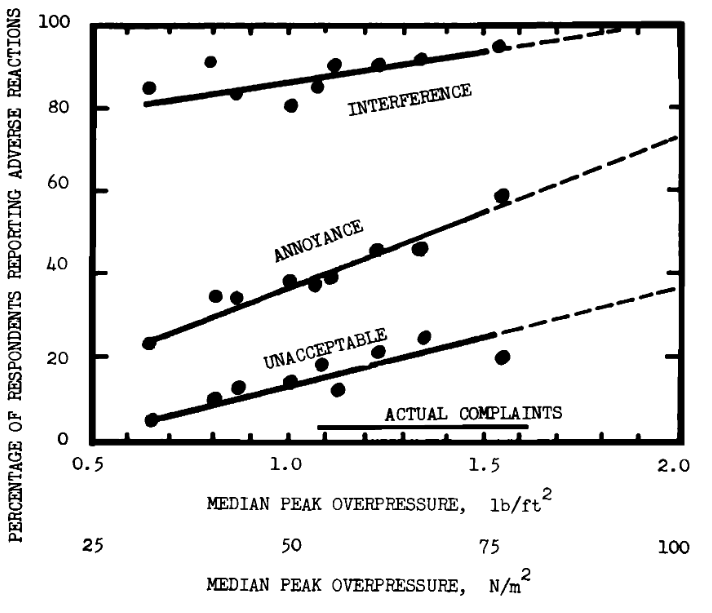
\includegraphics[width=0.7\linewidth]{figures/6_FlyBack/OverPressureResponse}
\caption{}
\label{fig:OverPressureResponse}
\end{figure}


\section{Alternate Launch Locations}

Southern Launch

note potential for sonic booms and safety issues




\section{Summary}
The fly-back trajectory of the SPARTAN hypersonic vehicle is investigated, from separation at 7.7$^\circ$S,145.0$^\circ$E to landing at 15.3$^\circ$S,144.9$^\circ$E, corresponding to a near 180$^\circ$ turn and a fly-back of 878km. The aerodynamics of the SPARTAN are calculated using CART3D, an inviscid CFD package, over the range of Mach numbers and angle of attack values of flight. The optimal trajectory of the SPARTAN is calculated, to fly-back to the initial launch position with minimum fuel. The optimal trajectory is calculated using the launch vehicle optimal control program LODESTAR. It is found that the SPARTAN is capable of returning to its initial launch position, using 166.0kg of fuel. The optimal trajectory terminates when SPARTAN reaches 200m altitude at a velocity of 119.8m/s. After this point, it is assumed that the SPARTAN lands on a traditional runway, at similar conditions to the space shuttle.  
This result indicates that the fly-back of a hypersonic launch vehicle from high velocity separation at a Mach number greater than nine, returning to its initial launch site using scramjet hypersonic airbreathing engines, is feasible. This fly-back to the the original launch site is a crucial component for low cost access-to-space using scramjets. 

The coefficient of drag of the SPARTAN and specific impulse of the scramjet engines were independently varied by $\pm10\%$ and the new optimal trajectories calculated to assess the robustness of the fly-back trajectory to uncertainties in vehicle aerodynamics and scramjet performance. It was found that a $\pm10\%$ variation in $C_D$ results in a +31.0\% or -34.9\% variation in fuel mass burned during fly-back, while a $\pm10\%$ variation in $I_{SP}$ results in a much smaller variation of -6.9\% or +13.8\%. These results indicate that the aerodynamics of a fly-back hypersonic accelerator are much more significant to the fly-back fuel usage than the performance of the scramjet engine. 

